\chapter{电子光谱与光物理}\label{ch:b3:electronic-spectroscopy}

在酒吧昏暗的紫外灯下，一杯汤力水
泛着淡淡的、幽灵般的蓝光。其中所含的奎宁吸收紫外光，
而人眼看不见紫外光，奎宁几纳秒后将其中一部分以可见蓝光的形式放出。
吸收、激发态的短暂寿命、较长波长处的发射、
以及未以光的形式释放出的能量：激发分子的命运
是各速率常数不同的过程之间的竞争，
其光谱由分子的振动以及
\cref{ch:b3:group-theory-applied}中的对称性规则决定。本章研究电子跃迁
及其之后发生的过程，这一学科称为光物理学；
\cref{ch:b3:photochemistry}补充了激发
分子发生反应的情形。

\begin{recall}
本科一年级分册用比尔–朗伯定律测量了吸光度，$A =
\varepsilon\ell c$，定义了摩尔吸光系数、发色团与
共轭体系，并将颜色与最大吸收波长联系起来。本科二年级分册
命名了前线轨道 HOMO 和 LUMO。在\Cref{ch:b3:many-electron-atoms}
中定义了单重态和三重态；在\cref{ch:b3:group-theory-applied}
中给出了消失积分定理；在\cref{ch:b3:rovibrational-spectroscopy}
中讨论了化学键的振动能级。
\end{recall}

\begin{omfigure}
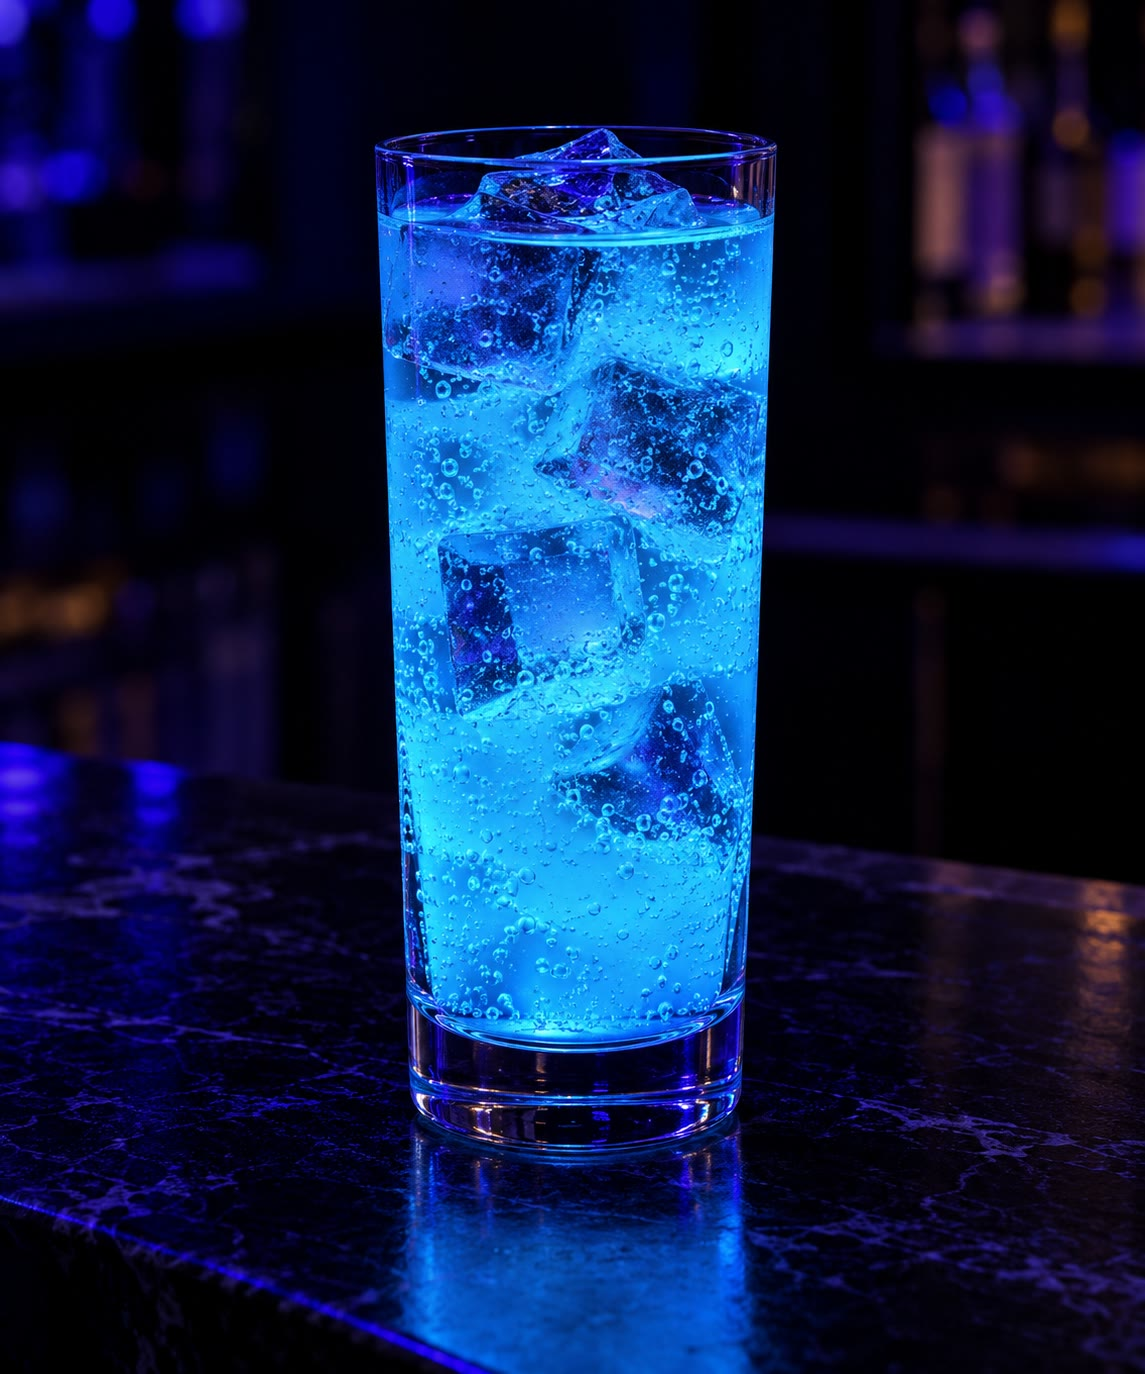
\includegraphics[height=4.6cm]{images/book4/ai/b3-07-tonic.jpg}\hspace{1em}%
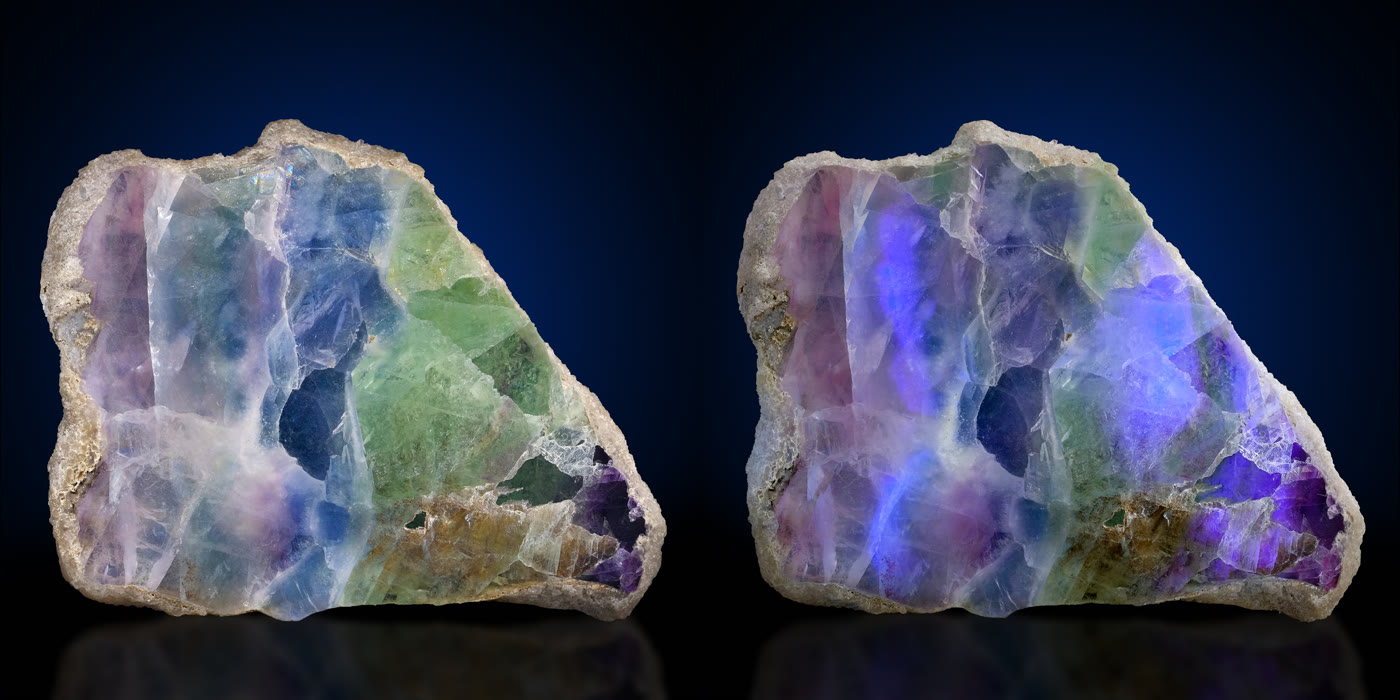
\includegraphics[height=4.6cm]{images/book4/fluorite-uv.jpg}

{\small 左：汤力水在紫外灯下发出蓝光。右：
日光下的萤石，以及其在紫外光下发出的荧光，荧光一词即由该矿物得名。
摄影：Masha Milshina，CC BY 4.0。}
\end{omfigure}

\section{电子跃迁及其选择定则}

\begin{definition}[跃迁偶极矩、振子强度]\label{def:b3:electronic-spectroscopy:transition-dipole}
两态之间的\emph{跃迁偶极矩}\index{跃迁偶极矩}
为 $\Psi_i$ 与 $\Psi_f$ 之间的 $\boldsymbol\mu_{fi} = \langle\Psi_f|\hat{\boldsymbol\mu}|\Psi_i
\rangle$，其中 $\hat{\boldsymbol\mu} = -e\sum_k\mathbf r_k$（加上原子核的电荷，
它们在正交态之间相消）。\emph{振子
强度}\index{振子强度}$f$ 是衡量吸收带强度的
无量纲的量，对最强的跃迁约为 1。
\end{definition}

\begin{proposition}[吸收强度与振子强度]\label{prop:b3:electronic-spectroscopy:intensity}
吸收带的积分吸收与 $|\boldsymbol\mu_{fi}|^2$ 成正比，
而实际上
\[
f \approx 4.32\times10^{-9}\int\varepsilon(\tilde\nu)\,\dd\tilde\nu,
\]
式中 $\varepsilon$ 的单位为 \unit{L.mol^{-1}.cm^{-1}}，$\tilde\nu$ 的单位为 \unit{cm^{-1}}。
\end{proposition}
\admitted

比例关系来自含时微扰理论，而数值因子来自经典振子，
两者都将在更高级的课程中讨论。这里重要的是
$f$ 只有在 $\boldsymbol\mu_{fi}$ 大时才大，
而对称性可以使其为零。

\begin{theorem}[自旋选择定则]\label{thm:b3:electronic-spectroscopy:spin-rule}
在总自旋不同的两态之间的电偶极跃迁
是禁阻的：$\Delta S = 0$。
\end{theorem}

\begin{proof}
每个态都是空间函数与自旋函数的乘积，$\Psi = \phi\,\chi$。
偶极算符只作用于位置，因此 $\langle\phi_f\chi_f|\hat{\boldsymbol\mu}|
\phi_i\chi_i\rangle = \langle\phi_f|\hat{\boldsymbol\mu}|\phi_i\rangle\langle\chi_f|\chi_i\rangle$.
不同 $S$ 的自旋函数是 $\hat S^2$ 的本征函数，其
本征值各不相同，因此二者正交（由\cref{thm:b3:quantum-model-systems:hermitian-real}可知）：
因而第二个因子为零。
\end{proof}

\begin{theorem}[拉波特规则]\label{thm:b3:electronic-spectroscopy:laporte}
在具有反演中心的分子中，电偶极跃迁必须
改变宇称：$g \leftrightarrow u$ 是允许的，$g \leftrightarrow g$ 与 $u
\leftrightarrow u$ 均被禁阻。这就是\emph{拉波特规则}\index{拉波特规则}。
\end{theorem}

\begin{proof}
$\hat{\boldsymbol\mu}$ 的各分量在反演下变号，它们属于 $u$。
乘积 $\Gamma_f\otimes\Gamma_\mu\otimes\Gamma_i$ 属于 $g$，当且仅当 $\Gamma_f$ 与 $\Gamma_i$
宇称相反；否则它属于 $u$，因而不能包含全对称
表示（由\cref{thm:b3:group-theory-applied:vanishing-integral}可知）。
\end{proof}

两条规则对理想化的态严格成立；实际分子会放宽它们，
——自旋–轨道耦合使单重态与三重态的成分混合，振动
使分子在瞬间失去对称中心——于是“禁阻”
跃迁便会出现，且较弱。八面体配合物的 $d$--$d$ 吸收带，
均为拉波特禁阻且较弱，其颜色正是源于这种放宽，
（见\cref{ch:b3:complex-spectra-magnetism}）。

\begin{definition}[电荷转移跃迁]\label{def:b3:electronic-spectroscopy:charge-transfer}
\emph{电荷转移跃迁}\index{电荷转移跃迁}是将电子从
主要定域于体系某一部分的轨道（施主）迁移到
主要定域于另一部分的轨道（受主）上的过程；其跃迁偶极矩
很大，吸收带强而宽，能量对溶剂的
极性十分敏感。
\end{definition}

\begin{method}[吸收带的指认]\label{met:b3:electronic-spectroscopy:assign-band}
\begin{enumerate}
  \item $\varepsilon_{\max}$ 大于约 \qty{e4}{L.mol^{-1}.cm^{-1}}：允许的
        跃迁（共轭体系的 $\pi\to\pi^*$，或电荷转移）。
  \item $\varepsilon_{\max}$ 为 10 至几百：禁阻的（$n\to\pi^*$，
        对称性禁阻；$d$--$d$，拉波特禁阻）。
  \item $\varepsilon_{\max}$ 小于 1：自旋禁阻。
  \item $n\to\pi^*$ 吸收带在质子性溶剂中向短波方向移动
        （孤电子对因氢键而稳定化），$\pi\to\pi^*$ 吸收带
        通常向长波方向移动。
\end{enumerate}
\end{method}

\section{弗兰克–康登原理}

\begin{theorem}[弗兰克–康登原理]\label{thm:b3:electronic-spectroscopy:franck-condon}
在玻恩–奥本海默近似下，若跃迁偶极矩
几乎不依赖核的位置，则由下电子态的振动能级 $v''$
跃迁到上电子态的振动能级 $v'$ 的电子振动跃迁强度，
正比于 $|\langle\chi_{v'}|\chi_{v''}\rangle|^2$，
即两个振动波函数交叠积分的平方：称此为\emph{弗兰克–康登原理}\index{弗兰克–康登原理}。
电子跃迁是竖直的：
跃迁时核保持不动，而电子发生跃迁。
\end{theorem}

\begin{proof}
取 $\Psi = \psi_{\mathrm{el}}(\mathbf r;R)\chi_v(R)$，则跃迁矩为
$\int\chi_{v'}^*\big[\int\psi'^*_{\mathrm{el}}\hat\mu\psi''_{\mathrm{el}}\dd\mathbf r\big]
\chi_{v''}\,\dd R$。方括号中的量即电子跃迁矩
$\mu_{\mathrm{el}}(R)$；取其为常数（康登近似），它可提到积分号外，
得 $\mu_{\mathrm{el}}\langle\chi_{v'}|\chi_{v''}\rangle$。
\end{proof}

\begin{definition}[电子振动跃迁、电子振动谱带序列、弗兰克–康登因子]\label{def:b3:electronic-spectroscopy:vibronic}
同时改变电子态与振动态的跃迁，称为\emph{电子振动跃迁}\index{电子振动跃迁}；
谱线 $v' \leftarrow 0$（$v' = 0, 1, 2,
\dots$）构成一个\emph{电子振动谱带序列}\index{电子振动谱带序列}；
某一电子振动谱线的\emph{弗兰克–康登因子}\index{弗兰克–康登因子}为
$|\langle\chi_{v'}|\chi_{v''}\rangle|^2$。
\end{definition}

\begin{proposition}[位移振子]\label{prop:b3:electronic-spectroscopy:displaced}
若两个态都是频率相同的谐振子，且上态的极小点
位移了 $\Delta$（以 $\sqrt{\hbar/m\omega}$ 为单位），则从 $v'' = 0$ 出发的弗兰克–康登因子
构成泊松分布，
$|\langle v'|0\rangle|^2 = \eu^{-S}S^{v'}/v'!$，其中 $S = \Delta^2/2$；最强的谱线
位于 $v' = S$ 附近。
\end{proposition}
\admitted

一般情形的证明用到
\cref{ch:b3:quantum-model-systems}中的升降算符；本章图中的数据
通过直接积分检验了该公式。位移较小时只有
一条很强的 0--0 谱线；位移较大时为长的谱带序列，其中最强的谱线
远离 0--0 谱线。

\begin{omfigure}
\begin{tikzpicture}
\begin{axis}[name=pc, width=0.46\linewidth, height=6cm, xmin=-4, xmax=5, ymin=0,
  ymax=14, axis lines=left, xtick=\empty, ytick=\empty, xlabel={核坐标},
  ylabel={能量}, label style={font=\small}]
\addplot[black, thick] table[x=y, y=ground] {figdata/out/bachelor-3-franck-condon-curves.dat};
\addplot[omDef, thick] table[x=y, y=excited] {figdata/out/bachelor-3-franck-condon-curves.dat};
\draw[omabs] (axis cs:0,0.5) -- (axis cs:0,10.6);
\draw[omvib] (axis cs:-1,0.5) -- (axis cs:1,0.5);
\draw[omvib] (axis cs:0.732,9.5) -- (axis cs:2.732,9.5);
\draw[omvib] (axis cs:-0.000,10.5) -- (axis cs:3.464,10.5);
\draw[omvib] (axis cs:-0.504,11.5) -- (axis cs:3.968,11.5);
\draw[omvib] (axis cs:-0.914,12.5) -- (axis cs:4.378,12.5);
\node[font=\small, anchor=west] at (axis cs:-3.9,13.0) {激发态};
\node[font=\small, anchor=west] at (axis cs:3.0,1.5) {基态};
\node[font=\scriptsize, anchor=east] at (axis cs:-0.05,5.5) {竖直跃迁};
\end{axis}
\begin{axis}[at={(pc.east)}, anchor=west, xshift=1.3cm, width=0.46\linewidth,
  height=6cm, xmin=-0.5, xmax=12.5, ymin=0, ymax=0.8, axis lines=left, ycomb,
  xlabel={$v'$}, ylabel={弗兰克–康登因子}, label style={font=\small},
  tick label style={font=\small}]
\addplot[black, very thick] table[x=v, y=s03] {figdata/out/bachelor-3-franck-condon-sticks.dat};
\addplot[omDef, very thick, xshift=2pt] table[x=v, y=s15] {figdata/out/bachelor-3-franck-condon-sticks.dat};
\addplot[omThm, very thick, xshift=4pt] table[x=v, y=s5] {figdata/out/bachelor-3-franck-condon-sticks.dat};
\end{axis}
\end{tikzpicture}

{\small 左：从基态最低能级出发的竖直跃迁，
落在激发态曲线上，该曲线因键长增大而位移，此处远高于
其极小点（取 $S = 1.5$）。右：$S = 0.3$（黑）、1.5（蓝）和 5（红）时谱带序列的
弗兰克–康登因子；每组之和
均为 1。}
\end{omfigure}

\begin{example}[碘]\label{ex:b3:electronic-spectroscopy:iodine}
% ledger: diat:I2.re, diat:I2B.re, diat:I2B.we, imass:I127
碘蒸气呈紫色，因为其 B$\leftarrow$X 吸收带吸收黄绿光。
键长由基态的 \qty{266.6}{pm} 增至
B 态的 \qty{302.5}{pm}。在位移振子模型中，取 B 态频率
（\qty{125.7}{cm^{-1}}），$\Delta R = \qty{35.8}{pm}$ 给出 $S \approx 15$：吸收为
长的谱带序列，其最强谱线止于 B 态的高振动能级，
其延续部分则进入解离连续谱。
\end{example}

\section{激发态的去向：雅布隆斯基图}

\begin{definition}[雅布隆斯基图]\label{def:b3:electronic-spectroscopy:jablonski}
\emph{雅布隆斯基图}\index{雅布隆斯基图}表示分子的电子态
（单重态 $S_0, S_1, S_2, \dots$ 排成一列，三重态 $T_1, T_2,
\dots$ 排成另一列）、它们的振动能级，以及连接它们的各个过程：
辐射过程用直线箭头，无辐射过程用波浪箭头表示。
\end{definition}

\begin{definition}[无辐射过程]\label{def:b3:electronic-spectroscopy:radiationless}
\emph{振动弛豫}\index{振动弛豫}通过碰撞使激发分子
回到其电子态的最低振动能级，
历时皮秒量级。\emph{内转换}\index{内转换}
是重数相同的态之间的无辐射跃迁
（$S_2 \to S_1$，$S_1 \to S_0$）；\emph{系间窜越}\index{系间窜越}
则是重数不同的态之间的跃迁
（$S_1 \to T_1$，$T_1 \to S_0$）。
\end{definition}

\begin{definition}[发光、荧光、磷光、斯托克斯位移]\label{def:b3:electronic-spectroscopy:luminescence}
\emph{发光}\index{发光}是激发分子发射光的过程。
\emph{荧光}\index{荧光}是自旋允许的发射，
通常为 $S_1 \to S_0$，速度快（纳秒量级）；\emph{磷光}\index{磷光}是自旋禁阻的发射，
通常为 $T_1 \to S_0$，速度慢（毫秒至
秒量级）。\emph{斯托克斯位移}\index{斯托克斯位移}是吸收与
发射极大值之间的能量差。
\end{definition}

\begin{omfigure}
\begin{tikzpicture}[font=\small, >=Stealth]
  \foreach \y/\l in {0/{$S_0$}, 3.4/{$S_1$}, 5.6/{$S_2$}}{
    \draw[omstate] (0,\y) -- (3.6,\y); \node[anchor=east] at (-0.1,\y) {\l};
    \foreach \d in {0.25,0.5,0.75}{\draw[omvib] (0,\y+\d) -- (3.6,\y+\d);}}
  \draw[omstate] (5.0,2.5) -- (7.6,2.5); \node[anchor=west] at (7.7,2.5) {$T_1$};
  \foreach \d in {0.25,0.5,0.75}{\draw[omvib] (5.0,2.5+\d) -- (7.6,2.5+\d);}
  \draw[omabs] (0.3,0) -- (0.3,4.15) node[pos=0.35, left, font=\scriptsize, align=right] {吸收};
  \draw[omabs] (0.7,0) -- (0.7,5.85);
  \draw[omnonrad] (1.05,5.85) -- (1.05,5.6);
  \draw[omnonrad] (1.05,5.6) -- (1.05,3.4) node[pos=0.5, right, font=\scriptsize] {内转换};
  \draw[omnonrad] (0.45,4.15) -- (0.45,3.42);
  \draw[omfluo] (1.7,3.4) -- (1.7,0.5) node[pos=0.5, right, font=\scriptsize, align=left] {荧光};
  \draw[omnonrad] (3.2,3.4) -- (3.2,0.02) node[pos=0.5, right, font=\scriptsize] {内转换};
  \draw[omisc] (3.6,3.4) -- (5.0,3.1) node[pos=0.5, above, font=\scriptsize] {系间窜越};
  \draw[omnonrad] (5.3,3.1) -- (5.3,2.52);
  \draw[omphos] (6.0,2.5) -- (6.0,0.5) node[pos=0.5, right, font=\scriptsize, align=left] {磷光};
  \draw[omisc] (5.6,2.5) -- (3.7,0.02) node[pos=0.45, above left, font=\scriptsize, inner sep=1pt] {系间窜越};
  \draw[omvib, dashed] (3.6,0.5) -- (6.0,0.5);
  \draw[omvib, dashed] (3.6,0.0) -- (7.6,0.0);
\end{tikzpicture}

{\small 雅布隆斯基图。直箭头：吸收（蓝色）、荧光（红色）、
磷光（橙色）；波浪箭头：振动弛豫和
内转换（IC）；虚线波浪箭头：系间窜越（ISC）。
发射始于 $S_1$ 或 $T_1$ 的最低振动能级，
并可终止于 $S_0$ 的任一能级。}
\end{omfigure}

\begin{proposition}[卡莎规则]\label{prop:b3:electronic-spectroscopy:kasha}
除极少数例外，发光总是来自同一自旋多重度中的最低激发态
（$S_1$ 或 $T_1$），与最初被激发到哪个态无关：
\emph{卡莎规则}\index{卡莎规则}。
\end{proposition}
\begin{proof}[说明]
该规律由实验确立；其原因在于，位于较高激发态之间的
内转换（这些态彼此靠得很近）远快于发射，
而 $S_1$--$S_0$ 能隙较大。
\end{proof}

\begin{proposition}[镜像关系]\label{prop:b3:electronic-spectroscopy:mirror}
若激发态与基态具有相似的振动结构，则
荧光带是第一吸收带关于它们共同的
0--0 线的镜像；发射位于更长波长处（斯托克斯位移）。
\end{proposition}

\begin{proof}
吸收由 $v'' = 0$ 跃迁至各振动能级 $v'$（均属 $S_1$），位于 $E_{00} + v'h\nu'$；发射
由 $v' = 0$ 跃迁至各振动能级 $v''$（均属 $S_0$），位于 $E_{00} - v''h\nu''$。
若两者频率相同且弗兰克–康登因子相同（位移相等），
则两个振动序列关于 $E_{00}$ 对称。
\end{proof}

\begin{omfigure}
\begin{tikzpicture}
\begin{axis}[width=0.75\linewidth, height=5cm, xmin=17, xmax=33, ymin=0,
  ymax=1.15, axis x line=bottom, axis y line=left, ytick=\empty,
  xlabel={波数 / $10^3$ cm$^{-1}$}, ylabel={强度},
  legend cell align=left, legend style={font=\small, draw=none, at={(0.02,0.97)}, anchor=north west},
  tick label style={font=\small}, label style={font=\small}]
\addplot[omDef, thick] table[x=nu, y=abs] {figdata/out/bachelor-3-photophysics-bands.dat};
\addlegendentry{吸收}
\addplot[omThm, thick] table[x=nu, y=em] {figdata/out/bachelor-3-photophysics-bands.dat};
\addlegendentry{荧光}
\draw[gray, dashed] (axis cs:25,0) -- (axis cs:25,1.12);
\node[font=\scriptsize, gray, anchor=south west] at (axis cs:25,1.0) {0--0};
\end{axis}
\end{tikzpicture}

{\small 某模型分子的吸收光谱与荧光光谱（$S = 1$，振动
量子 \qty{1400}{cm^{-1}}）：关于 0--0 线互为镜像；
两极大值之间的间隔即为斯托克斯位移。}
\end{omfigure}

\section{激发态动力学}

激发后，$S_1$ 的布居数通过其所有可进行的过程衰减，
各过程均为一级：辐射衰变 $k_r$、内转换 $k_{\mathrm{IC}}$、
系间窜越 $k_{\mathrm{ISC}}$。

\begin{definition}[激发态寿命、辐射寿命]\label{def:b3:electronic-spectroscopy:lifetime}
\emph{激发态寿命}\index{激发态寿命}为 $\tau =
1/\sum k$，即激发态布居数的指数衰减
的时间常数。\emph{辐射寿命}\index{辐射寿命} $\tau_r =
1/k_r$ 是该态若以发射为其唯一去路时所具有的
寿命。
\end{definition}

\begin{definition}[量子产率]\label{def:b3:electronic-spectroscopy:quantum-yield}
紧随光吸收之后发生的某一过程的\emph{量子产率}\index{量子产率}，
等于该过程发生的次数除以所吸收的光子数。
\emph{荧光量子产率}\index{荧光量子产率} $\Phi_F$
为每吸收一个光子
所发射的荧光光子数。
\end{definition}

\begin{proposition}[量子产率与寿命]\label{prop:b3:electronic-spectroscopy:quantum-yield}
$\Phi_F = k_r/(k_r + k_{\mathrm{IC}} + k_{\mathrm{ISC}}) = k_r\tau = \tau/\tau_r$；同理
$\Phi_{\mathrm{ISC}} = k_{\mathrm{ISC}}\tau$，且各竞争过程的产率
之和为 1。
\end{proposition}

\begin{proof}
$\dd[S_1]/\dd t = -(k_r + k_{\mathrm{IC}} + k_{\mathrm{ISC}})[S_1]$，于是 $[S_1] = [S_1]_0\eu^{-t/\tau}$。
发射的光子数为 $\int_0^\infty k_r[S_1]\,\dd t = k_r\tau[S_1]_0$，
占 $[S_1]_0$ 个激发分子的份额。对各 $k$ 作同样的积分即得各产率，
其和为 $\tau\sum k = 1$。
\end{proof}

\begin{definition}[荧光猝灭剂、动态猝灭与静态猝灭]\label{def:b3:electronic-spectroscopy:quencher}
\emph{荧光猝灭剂}\index{荧光猝灭剂}是一种
使荧光减弱的物质。在\emph{动态猝灭}\index{动态猝灭}中，
它通过碰撞使激发分子失活，附加速率 $k_q[Q]$，
并缩短寿命；在\emph{静态猝灭}\index{静态猝灭}中，它
与基态分子形成不发荧光的配合物，使
荧光强度降低，而仍在发光的分子的寿命不变。
\end{definition}

\begin{theorem}[斯特恩–福尔默方程]\label{thm:b3:electronic-spectroscopy:stern-volmer}
对于动态猝灭，
\[
\frac{I_0}{I} = \frac{\tau_0}{\tau} = 1 + k_q\tau_0[Q] = 1 + K_{SV}[Q],
\]
称为\emph{斯特恩–福尔默方程}\index{斯特恩–福尔默方程}，其中 $I_0$、$\tau_0$
均在无猝灭剂时测得，$K_{SV} = k_q\tau_0$。
\end{theorem}

\begin{proof}
有猝灭剂时，$\tau = 1/(k_0 + k_q[Q])$，其中 $k_0 = 1/\tau_0$，故 $\tau_0/\tau = 1 +
k_q\tau_0[Q]$。荧光强度正比于 $\Phi_F = k_r\tau$，于是 $I_0/I = \tau_0/\tau$。
\end{proof}

\begin{omfigure}
\begin{tikzpicture}
\begin{axis}[name=dec, width=0.5\linewidth, height=5cm, xmin=0, xmax=40, ymode=log,
  ymin=0.005, ymax=1.2, axis lines=left, xlabel={$t$ / ns}, ylabel={$I(t)/I(0)$},
  legend cell align=left, legend style={font=\scriptsize, draw=none, at={(0.98,0.98)}, anchor=north east},
  tick label style={font=\small}, label style={font=\small}]
\addplot[black, thick] table[x=t, y=q0] {figdata/out/bachelor-3-photophysics-decays.dat};
\addlegendentry{$[Q] = 0$}
\addplot[omDef, thick] table[x=t, y=q1] {figdata/out/bachelor-3-photophysics-decays.dat};
\addlegendentry{0.01 M}
\addplot[omProp, thick] table[x=t, y=q2] {figdata/out/bachelor-3-photophysics-decays.dat};
\addlegendentry{0.02 M}
\addplot[omThm, thick] table[x=t, y=q4] {figdata/out/bachelor-3-photophysics-decays.dat};
\addlegendentry{0.04 M}
\end{axis}
\begin{axis}[at={(dec.east)}, anchor=west, xshift=1.4cm, width=0.42\linewidth,
  height=5cm, xmin=0, xmax=0.045, ymin=0, ymax=3.3, axis lines=left,
  xlabel={$[Q]$ / mol L$^{-1}$}, ylabel={$I_0/I = \tau_0/\tau$},
  xticklabel style={/pgf/number format/fixed, /pgf/number format/precision=2},
  scaled x ticks=false, tick label style={font=\small}, label style={font=\small}]
\addplot[omThm, thick, mark=*] table[x=Q, y=I0I] {figdata/out/bachelor-3-photophysics-sv.dat};
\end{axis}
\end{tikzpicture}

{\small 模型荧光团的动态猝灭（$\tau_0 = \qty{10}{ns}$，$k_q =
\qty{5e9}{L.mol^{-1}.s^{-1}}$）。左图：荧光衰减曲线在对数坐标下呈直线，
猝灭剂越多，直线越陡。右图：斯特恩–福尔默直线，斜率为
$K_{SV} = k_q\tau_0 = \qty{50}{L/mol}$。}
\end{omfigure}

\begin{method}[相对荧光量子产率]\label{met:b3:electronic-spectroscopy:relative-yield}
\begin{enumerate}
  \item 选取已知 $\Phi_{\mathrm{std}}$ 的标准物质，
        其在相同激发波长处有吸收。
  \item 配制稀溶液（$A < 0.1$，以避免再吸收），
        并在相同
        条件下记录其吸光度 $A$ 与积分发射光谱 $F$。
  \item $\Phi = \Phi_{\mathrm{std}}\,\dfrac{F}{F_{\mathrm{std}}}\,\dfrac{A_{\mathrm{std}}}{A}\,
        \dfrac{n^2}{n_{\mathrm{std}}^2}$，末项用于校正
        溶剂折射率的影响。
\end{enumerate}
\end{method}

\begin{method}[猝灭数据的分析]\label{met:b3:electronic-spectroscopy:stern-volmer}
\begin{enumerate}
  \item 以 $I_0/I$ 对 $[Q]$ 作图，若得过 1 的直线，则其斜率为 $K_{SV}$。
  \item 同时测量寿命：若 $\tau_0/\tau$ 落在同一直线上，
        则为动态猝灭，且 $k_q = K_{SV}/\tau_0$；若 $\tau$ 不变，则为静态猝灭。
  \item 将 $k_q$ 与扩散极限比较，该极限在水中约为 \qty{e10}{L.mol^{-1}.s^{-1}}
        （见\cref{ch:b3:rate-theories}）：若 $k_q$ 接近该值，
        则几乎每次相遇都会发生猝灭。
\end{enumerate}
\end{method}

\begin{example}[奎宁与蒽]\label{ex:b3:electronic-spectroscopy:quinine}
% ledger: fl:quinine.labs, fl:quinine.eps, fl:quinine.phi, fl:anthracene.labs, fl:anthracene.phi
硫酸奎宁溶于 \qty{0.5}{M} 硫酸中，在 \qty{349}{nm} 处有吸收，摩尔吸光系数 $\varepsilon =
\qty{5700}{L.mol^{-1}.cm^{-1}}$，并发荧光，$\Phi_F = 0.546$，这使其成为
测定相对量子产率的经典标准物。蒽在环己烷中
在 \qty{356}{nm} 处有吸收，$\Phi_F = 0.36$；未发荧光的激发分子
大多转入三重态。
\end{example}

\section{应用}

荧光在暗背景下检测，这使荧光分析法
灵敏度比吸收光谱法高出百倍至千倍：
纳摩尔浓度的荧光化合物可以常规测定。
荧光探针通过其波长、
产率或寿命反映所处环境（极性、pH、离子的结合）；
两个荧光团之间的能量传递仅在几纳米范围内有效，可用来
测定蛋白质中的距离。重金属的磷光配合物，其中
自旋–轨道耦合使系间窜越高效，从而捕获三重态
于显示屏的发光二极管中。

\begin{inthelab}[时间相关单光子计数]
为测量纳秒寿命，样品由脉冲激光二极管
以兆赫兹重复频率激发，每个脉冲记录
首个被探测到的荧光光子的延迟。经过数百万次脉冲后，
延迟直方图即为衰减曲线，由此拟合出 $\tau$，
仪器响应在散射溶液上测定。紫外线
光源被封闭；操作者佩戴能阻挡其
波长的护目镜。
\end{inthelab}

\begin{history}[斯托克斯，1852 年]
乔治·加布里埃尔·斯托克斯让太阳光通过紫色玻璃和棱镜，
射入奎宁溶液，看到蓝光从被
不可见紫外线照亮的区域射出：发射光总
是比吸收光波长更长。他将这种现象命名为荧光，
取自同样会发光的萤石矿物。
\end{history}

\section{练习}

\begin{exercise}[$\star$]\label{exo:b3:electronic-spectroscopy:1}
判断下列跃迁是否允许，并说明所依据的规则：（a）苯中的 $S_0 \to T_1$；（b）八面体配合物的 $d$--$d$
跃迁；（c）乙烯的 $\pi\to\pi^*$ 跃迁
（$B_{1u} \leftarrow A_g$，在 $D_{2h}$ 中）；（d）甲醛的 $n\to\pi^*$ 跃迁
（$A_2$）？
\end{exercise}

\begin{exercise}[$\star$]\label{exo:b3:electronic-spectroscopy:2}
一种化合物在 \qty{349}{nm} 处吸收，并在
\qty{450}{nm} 处有荧光极大（习题数据）。计算其斯托克斯位移，分别以 \unit{cm^{-1}}
和 eV 为单位。
\end{exercise}

\begin{exercise}[$\star$]\label{exo:b3:electronic-spectroscopy:3}
% ledger: fl:quinine.eps
计算 \qty{1.0e-5}{mol/L} 硫酸奎宁溶液在 \qty{349}{nm} 处的吸光度，
所用比色皿光程为 \qty{1}{cm}，并求其吸收的光所占比例。
\end{exercise}

\begin{exercise}[$\star$]\label{exo:b3:electronic-spectroscopy:4}
某荧光团 $\Phi_F = 0.60$，$\tau = \qty{4.0}{ns}$。计算 $k_r$、
辐射寿命以及非辐射速率常数之和。
\end{exercise}

\begin{exercise}[$\star\star$]\label{exo:b3:electronic-spectroscopy:5}
某谱带为高斯型，$\varepsilon_{\max} = \qty{5700}{L.mol^{-1}.cm^{-1}}$，半高宽为
\qty{5000}{cm^{-1}}。估算其振子强度（高斯函数的积分为
$1.0645\,\varepsilon_{\max}\times$半高宽）。
\end{exercise}

\begin{exercise}[$\star\star$]\label{exo:b3:electronic-spectroscopy:6}
对于位移振子，求 $S = 0.3$、1.5 和 5 时电子振动谱带序列中最强的谱线，
并求其因子与 0--0 谱线因子之比。
\end{exercise}

\begin{exercise}[$\star\star$]\label{exo:b3:electronic-spectroscopy:7}
自 $S_1$ 出发，$k_r = \qty{1.0e8}{s^{-1}}$，$k_{\mathrm{IC}} = \qty{2.0e7}{s^{-1}}$，$k_{\mathrm{ISC}} =
\qty{3.0e8}{s^{-1}}$。计算 $\tau$、$\Phi_F$ 和 $\Phi_{\mathrm{ISC}}$。
\end{exercise}

\begin{exercise}[$\star\star$]\label{exo:b3:electronic-spectroscopy:8}
% ledger: fl:quinine.phi, nD:water, nD:cyclohexane
蒽在环己烷中的荧光（$A = 0.040$）积分强度为
稀硫酸中硫酸奎宁（$A = 0.050$，$\Phi =
0.546$）的 0.46 倍。已知环己烷的折射率为 1.4266，
稀酸（水）的折射率为 1.333，计算蒽的 $\Phi_F$。
\end{exercise}

\begin{exercise}[$\star\star$]\label{exo:b3:electronic-spectroscopy:9}
荧光团在猝灭剂浓度分别为 0、0.010 和 \qty{0.020}{mol/L} 时，
其寿命分别为 8.0、5.6 和 \qty{4.3}{ns}。该猝灭是否为动态猝灭？
求 $K_{SV}$ 和 $k_q$。
\end{exercise}

\begin{exercise}[$\star\star\star$]\label{exo:b3:electronic-spectroscopy:10}
加入猝灭剂后荧光强度减半，而测得的寿命仍为 \qty{6.0}{ns}。
这属于哪一类猝灭？它对基态说明了什么？
写出 $I_0/I$ 与
配合物缔合常数之间的对应关系。
\end{exercise}

\begin{exercise}[$\star\star\star$]\label{exo:b3:electronic-spectroscopy:11}
% ledger: fl:anthracene.phi
蒽在环己烷中 $\Phi_F = 0.36$，在测量条件下
$\tau = \qty{5.0}{ns}$（习题数据），计算 $\tau_r$ 以及
内转换可忽略时的三重态产率。为什么
辐射寿命比实测寿命长？
\end{exercise}

\begin{exercise}[$\star\star\star$]\label{exo:b3:electronic-spectroscopy:12}
对于两个电子，单重态自旋函数为 $\frac{1}{\sqrt2}[\alpha\beta - \beta\alpha]$，
$M_S = 0$ 的三重态函数为 $\frac{1}{\sqrt2}[\alpha\beta + \beta\alpha]$。证明二者正交，
并就 $T_1 \leftarrow S_0$ 的强度
在无自旋–轨道耦合时作出结论。
\end{exercise}

\section{问题：为什么汤力水会发光}

\begin{problem}[{周末问题——奎宁的吸收、其激发态的去向、
氯离子引起的猝灭，以及
是否每次碰撞都会猝灭}]
\label{pb:b3:electronic-spectroscopy:1}
% ledger: fl:quinine.labs, fl:quinine.eps, fl:quinine.phi, visc:H2O.25C
硫酸奎宁溶于 \qty{0.5}{M} 硫酸中：吸收极大位于 \qty{349}{nm}，
$\varepsilon = \qty{5700}{L.mol^{-1}.cm^{-1}}$，$\Phi_F = 0.546$。题目数据：
无猝灭剂时荧光寿命为 $\tau_0 = \qty{19}{ns}$；发射极大位于 \qty{450}{nm} 附近；
加入氯化钠后得到如下强度比。
\begin{center}\small
\begin{tabular}{lccccc}
\hline
$[\ce{Cl-}]$ / mol L$^{-1}$ & 0 & 0.010 & 0.020 & 0.040 & 0.080 \\
$I_0/I$ & 1.000 & 1.594 & 2.188 & 3.376 & 5.752 \\ \hline
\end{tabular}
\end{center}
在 \qty{25}{\celsius} 下水的黏度为 \qty{0.890}{mPa.s}；$R =
\qty{8.314}{J.K^{-1}.mol^{-1}}$。

\medskip\noindent\textbf{第一部分——吸收。}
\begin{enumerate}
  \item 计算 \qty{1.0e-4}{mol/L} 溶液在 \qty{349}{nm} 处的吸光度，
        所用比色皿光程为 \qty{1}{cm}。
  \item 入射光中有多大比例被吸收？
  \item 该跃迁是否允许？利用 $\varepsilon$ 判断。
  \item 给出被吸收光子的能量，单位为 eV。
  \item 为什么人眼在汤力水中看不到吸收色？
  \item 用于荧光实验的溶液为何要保持 $A = 0.1$ 以下？
\end{enumerate}

\medskip\noindent\textbf{第二部分——激发态。}
\begin{enumerate}[resume]
  \item 画出自 $S_1$ 出发各过程的雅布隆斯基图。
  \item 计算辐射速率常数 $k_r$ 和辐射寿命。
  \item 计算非辐射速率常数之和。
  \item 以 \unit{cm^{-1}} 为单位计算斯托克斯位移。
  \item 吸收位于紫外区，为何发射光却呈蓝色？
  \item 计入每个光子的能量，被吸收能量中有多大比例
        以荧光形式发出？
\end{enumerate}

\medskip\noindent\textbf{第三部分——氯离子猝灭。}
\begin{enumerate}[resume]
  \item 以 $I_0/I$ 对 $[\ce{Cl-}]$ 作图，并检验其是否为线性。
  \item 用最小二乘法拟合五个数据点，确定 $K_{SV}$。
  \item 假设为动态猝灭，计算 $k_q$。
  \item 在 \qty{0.040}{mol/L} 时将测得怎样的寿命？
  \item 如何通过实验证明该猝灭是动态的？
  \item 汤力水不含氯离子，为什么它是奎宁
        发光的良好场所？
\end{enumerate}

\medskip\noindent\textbf{第四部分——每次碰撞都会猝灭吗？}
\begin{enumerate}[resume]
  \item 在黏度为 $\eta$ 的溶剂中，扩散控制的碰撞速率常数
        为 $k_d \approx 8RT/3\eta$。以 \unit{L.mol^{-1}.s^{-1}} 为单位计算它。
  \item 比较 $k_q$ 与 $k_d$。
  \item 有多大比例的碰撞会导致猝灭？
  \item 在黏度更大的溶剂中，猝灭会更快还是更慢？
  \item 给出结论：奎宁被氯离子猝灭时的比值
        $k_q/k_d$。
\end{enumerate}
\end{problem}
